\section{List of model features/parameters and their biological foundation}

To write:
\begin{itemize}
    \item Table of parameters
    \item Lower apical surface area
    \item Shape of boundary condition
    \item Cell types extracted from data
    \item differential adhesion
    \item Nematic l1 for closing off
\end{itemize}
\section{Visual closeness}
While the Drosophila embryo has been studied for decades, it is only relatively recently conputer vision has gotten to a point where quantitative analyses of 5000 is feasible. Therefore the most vital thing to recuperate is the visual agreement between the morphology of simulation and data.

On the following page, the simulation and corresponding frames from [stas' paper] can be seen and compared:

\newpage

\begin{figure}[H]
    \centering
    \vspace*{-1cm}\hspace*{-1cm}\makebox[\textwidth]{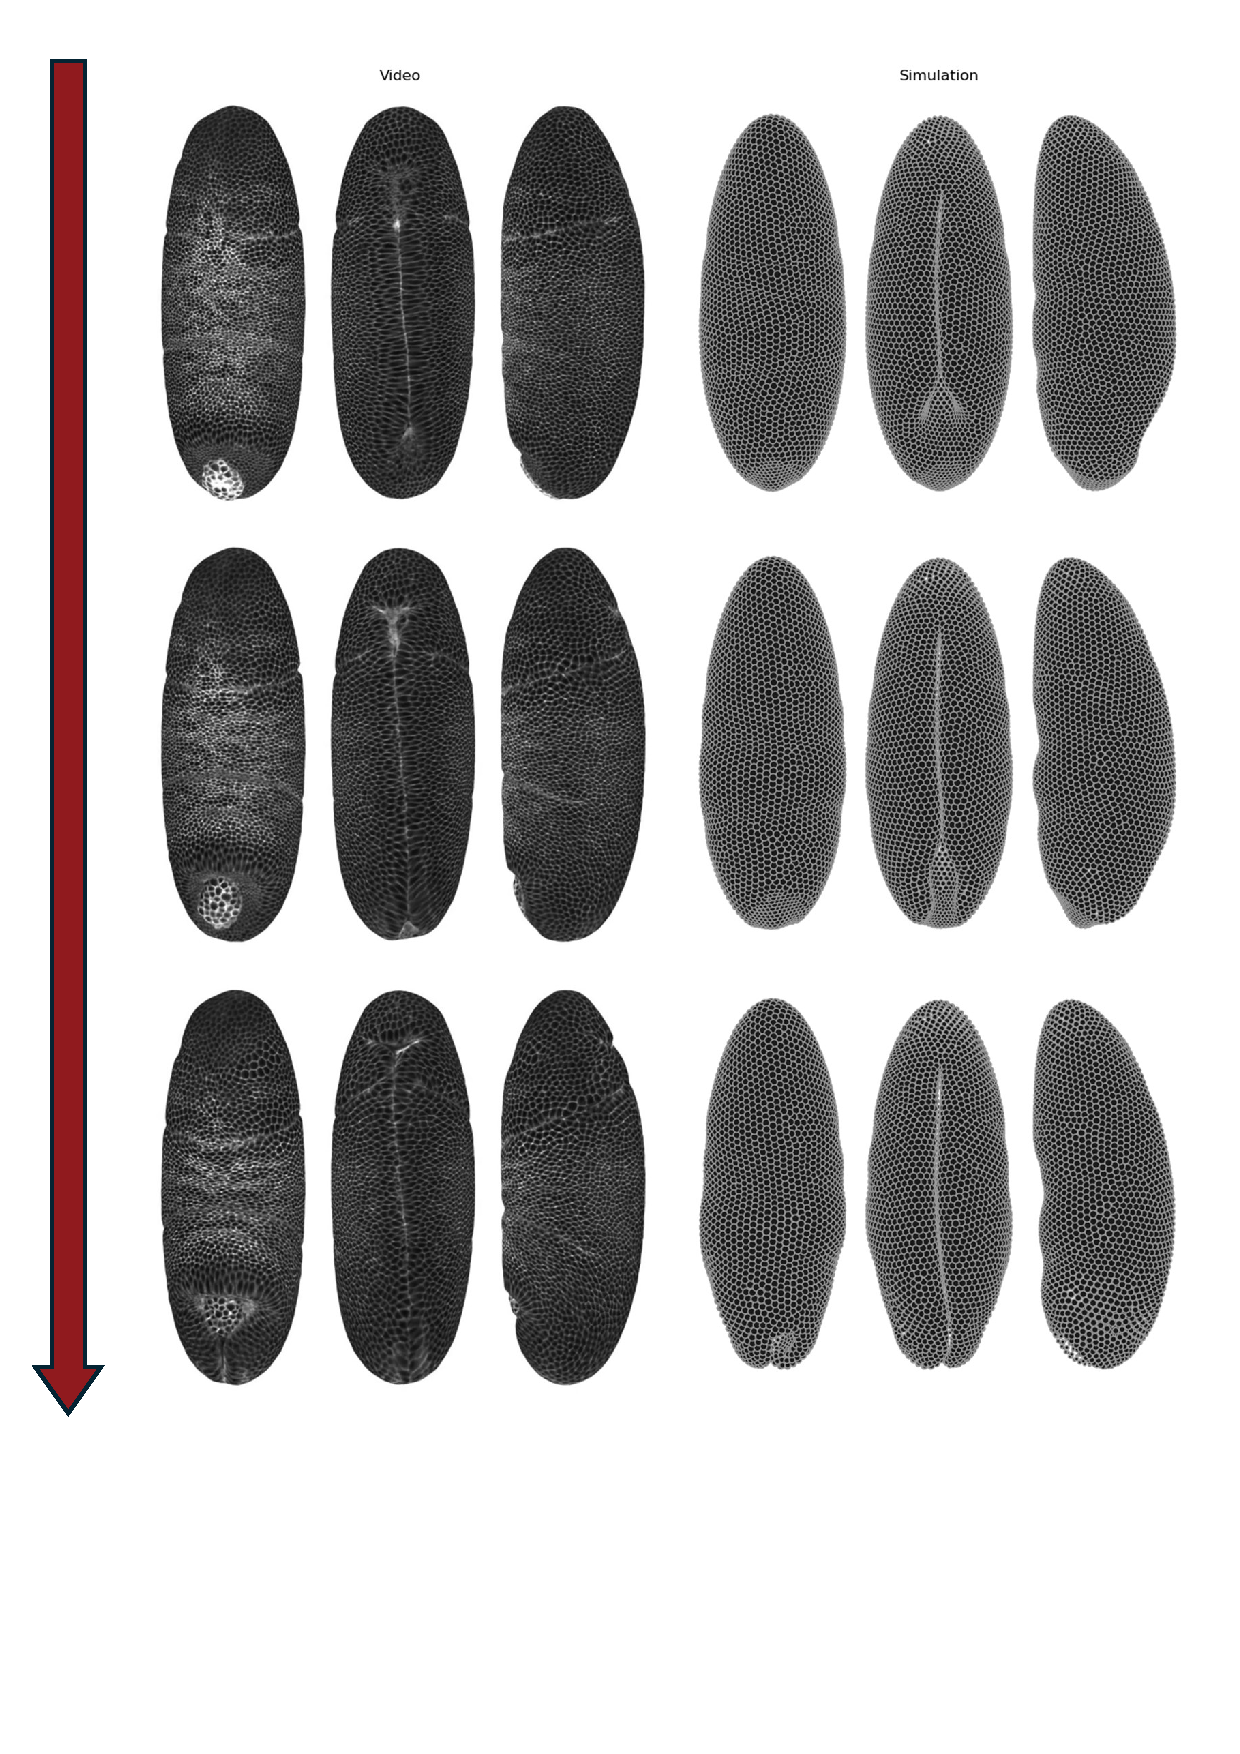
\includegraphics[width=0.85\paperwidth]{chapters/Results/figures/compare_to_vid_timeline.pdf}}
    \caption{Caption}
    \label{fig:enter-label}
\end{figure}
\newpage

\subsection{Ventral Furrow}
After mitosis stops, the the first visual change is on the belly, where a distinct cleft begins forming. \\

While all cells expressing \textit{twist} \& \textit{snail} lower their apical surface area, they do not constrict indiscriminately, instead starting with the \textit{inner} 8x60 cells.[citation needed] As the furrow closes off, creating closed-off tube with a recognizable light bulb-shape in the cross section, the tube extends dorsally.

In figure \ref{fig:VFComparison}, a comparison between a cross section of our simulation and in vivo imaging can be seen.

\begin{figure}[H]
    \centering
    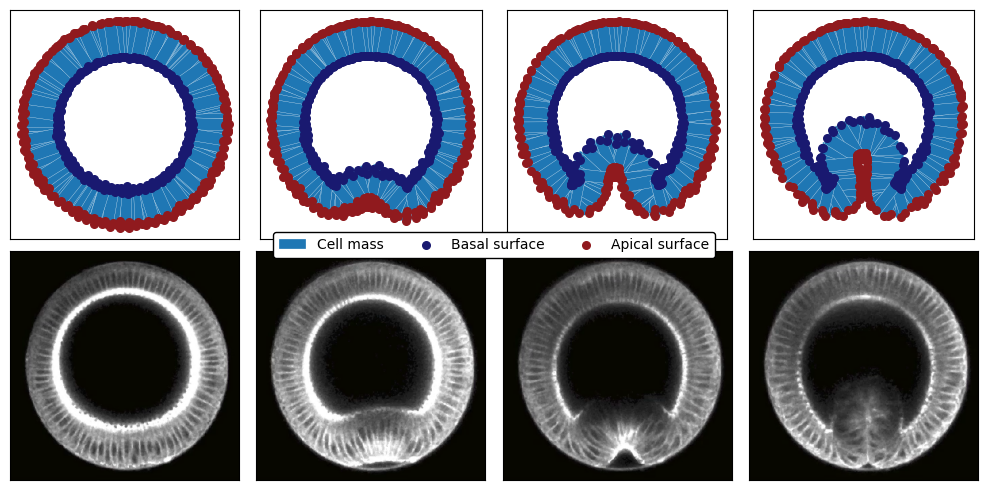
\includegraphics[width=1\linewidth]{chapters/Results/figures/VF_comparison.png}
    \caption{A comparison of simulation and frames from live development. \textbf{Upper row}: Simulation. \textbf{Lower row}: Multi-photon microscopy. \\Each frame is taken at equally spaced time intervals. Cross section video borrowed from \cite{conte2012biomechanical}}
    \label{fig:VFComparison}
\end{figure}


Maybe quantify here?
I am guessing we can do a cell-center fit?
Out of scope? Yes. Would be cool? Also yes.
\subsection{Germ band}
The Germ Band is defined as the YYY. The general consensus is, that the Germ Band is the main driver of dorsal motion, although it remains disputed.

If Figure \ref{fig:germbandCompare} a diagram of the motion of the Germ Band can be compared with the shape of the Germ Band in the first and last frame of our simulation. 

\begin{figure}[H]
    \centering
    \begin{subfigure}[b]{0.34\textwidth}
        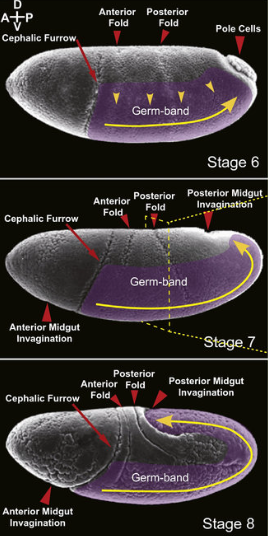
\includegraphics[width=\textwidth]{chapters/Results/figures/compareGB.png}
    \caption{Figure from \cite{kong2017forces} }
    \end{subfigure}
     \hfill
    \begin{subfigure}[b]{0.61\textwidth}
    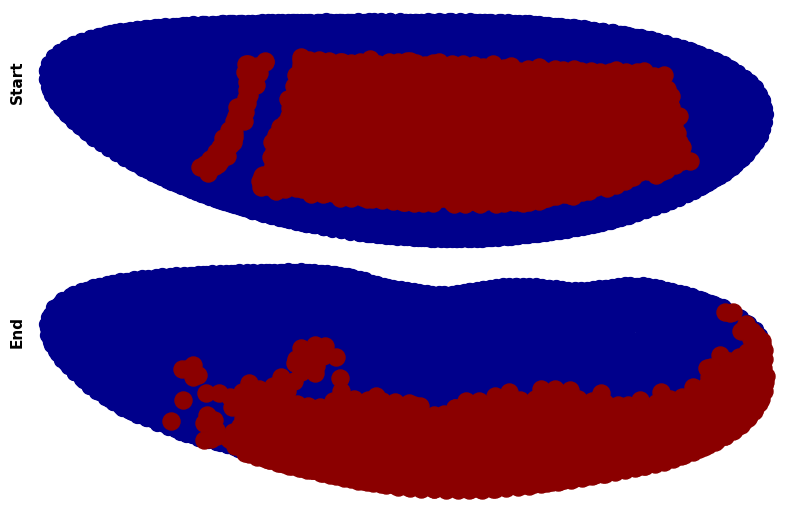
\includegraphics[width=\textwidth]{chapters/Results/figures/gb_firstframe_lastframe.png}
    \caption{Simulation}
    \end{subfigure}
    \caption{Colored in germ band for visual inspection.}
    \label{fig:germbandCompare}
\end{figure}

For an representation of the motions of the individual cells, see Figure \ref{fig:GBMovements} in the Appendix.
In general we see a great agreement between the morphological timeline of the germband between simulation and data.


\subsection{General morphology}
As way of visually seeing the changes in both local and global structure, drawing in straight lines before start of gastrulation and seeing how they translate and skew over time. An example of this (in both data and simulation can be seen in Figure \ref{fig:band-movements-stas}) 

\begin{figure}[H]
    \centering
    \makebox[\textwidth][c]{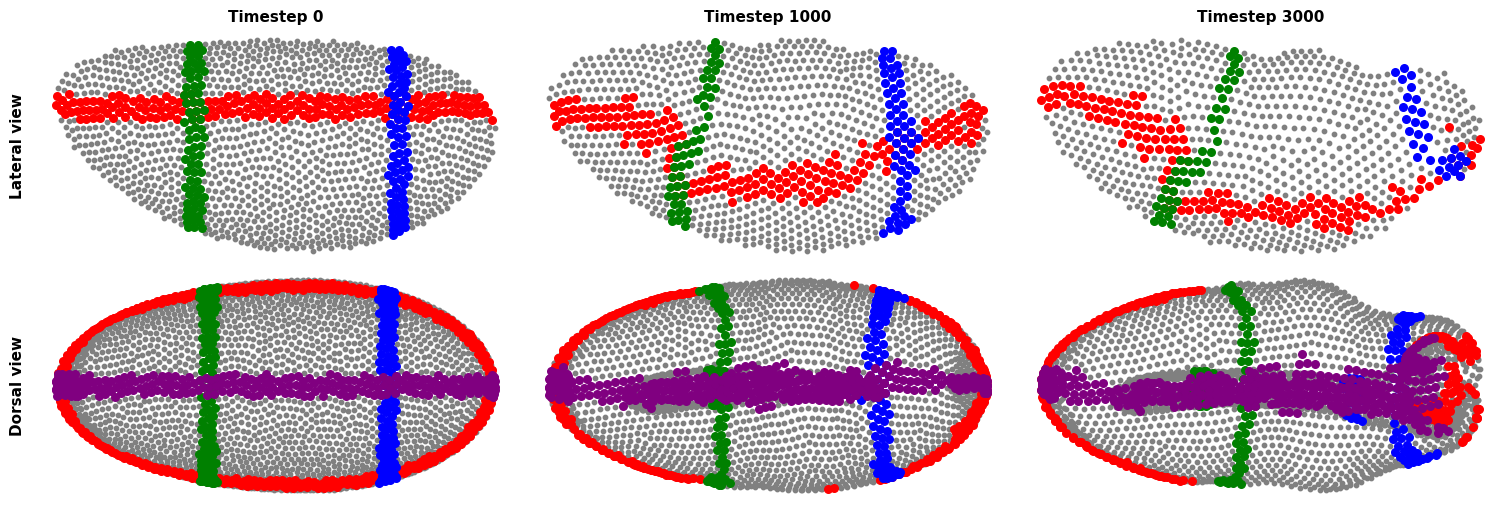
\includegraphics[width=1.1\linewidth]{chapters/Results/figures/band_movements.png}}
    % \caption{My simulation. Compare to figure \ref{fig:band-movements-stas}}
    % \label{fig:band-movements}
\end{figure}
\begin{figure}[H]
    \centering
    \makebox[\textwidth][c]{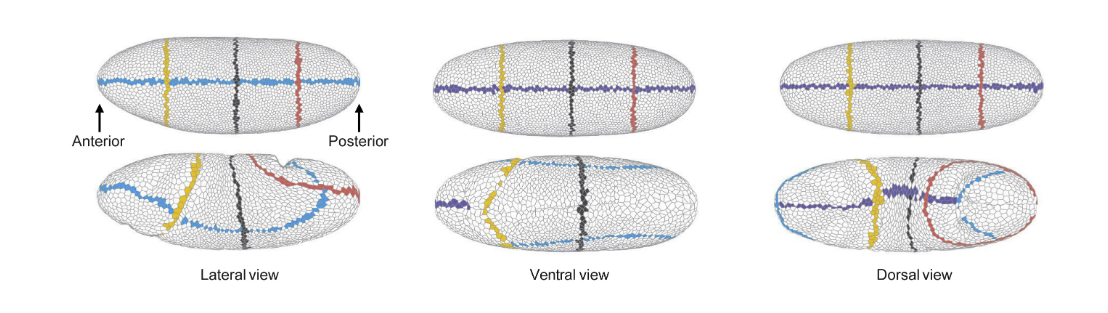
\includegraphics[width=1.\linewidth]{chapters/Results/figures/compareStasGBShape.png}}
    \caption{Position of specific bands over time.\\ \textbf{Top row:} Simulation | \textbf{Bottom row:}  Segmented images (from \cite{stern2022deconstructing}). \\TODO: make colors match.}
    \label{fig:band-movements-stas}
\end{figure}

As is evident, the general agreement is pretty good :)


\subsection{Auxiliary furrows}

In the absence of controlled folding of the dorsal tissue, the pressure from the extending germband, can lead to other folds(?) \url{https://brunovellutini.com/posts/cephalic-furrow-thread/}

This is key to both understanding why the invaginated posterior end does not travel further anteriorly.

Also the large scale morhpology change some runs had.
\subsection{Daniel}
\section{Quantitative closeness}
\subsection{Movements}
While comparing the large scale morphogenesis visually is interesting, for better quantification of the model performance, the following measure was devised:

For ever n'th time-step, look at the recent motion of each cell. Compare each of these to the average motion vector of the 10 spatially closest cells in data. The resulting angle difference between 0 and $\pi$ is scaled to be between 0 and 1, with 1 being perfect agreement.

\begin{figure}[H]
    \centering
    \makebox[\textwidth][c]{
    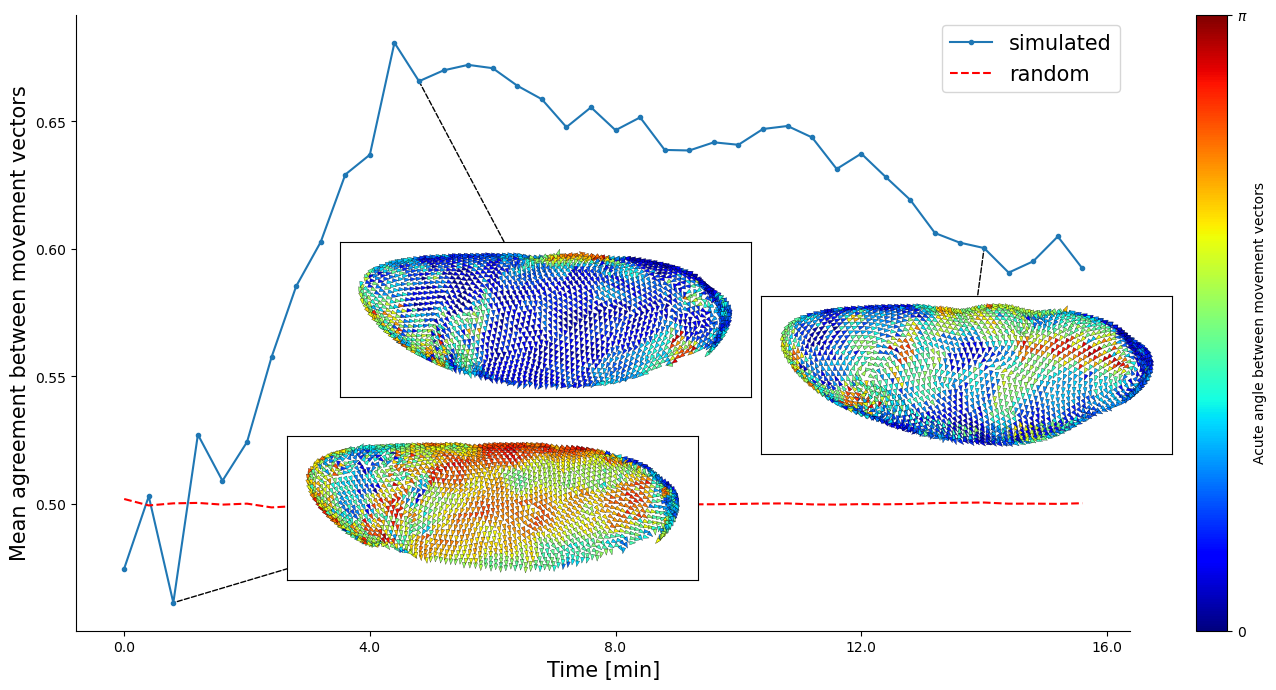
\includegraphics[width=1.3\linewidth]{chapters/Results/figures/movement_vectors_normal.png}
    }
    \caption{The motion-vector agreement across the full embryo as a function of time}
    \label{fig:enter-label}
\end{figure}

In general, we see a consistent, well-above average overlap. 


Important to note:
1) The data consist of machine-tracked cell positions. This means any radial motion is neglected.
2) Convergent extension is by its very nature based on the global motion being more important than the individual (see figure \ref{}) 

These two 



\subsection{Timing}
Cells have been shown to have remarkably precise internal clocks\footnote{cool footnote with a remarkable number\cite{cellinternal}} and chemical gradients in the embryo changing across timescales from seconds to hours\cite{shvartsman2008dynamics}. There is also the "biological clock"\cite{johanolsen2} that proteins themselves have dynamic structure that can change over time.\cite{johanolsen1}. But there is no evidence for any specific timing in stages 5-7 [citation needed]. The fact that our model seem have recapitulated much of the dynamics completely without any explicit time-dependent parameters seems to corroborate the fact that Boundary Conditions, Initial Conditions and an inter-atomic rule-set is sufficient for arbitrarily complex morphology/anatomy to arise. 


\subsection{Strain}

\begin{figure}[H]
    \centering
    \begin{subfigure}{0.45\linewidth}
        \centering
        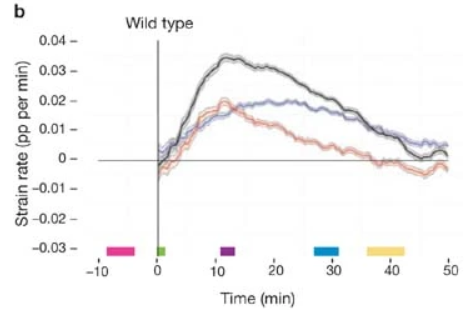
\includegraphics[width = \linewidth]{chapters/Results/figures/strain_rate_extrinsic.png}
    \end{subfigure}
        \begin{subfigure}{0.45\linewidth}
        \centering
        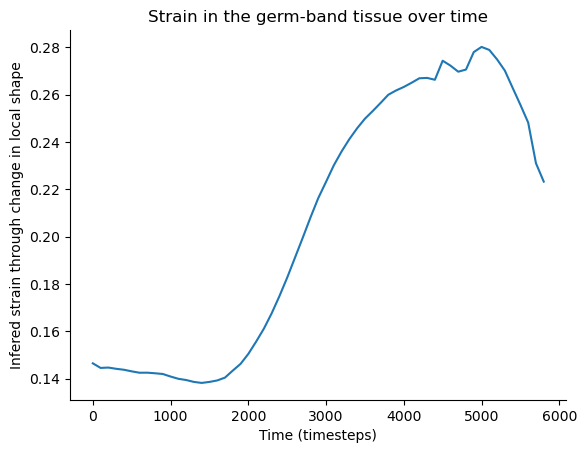
\includegraphics[width = \linewidth]{chapters/Results/figures/strain_smoothedpng.png}
    \end{subfigure}
    \label{fig:enter-label}
    \caption{Comparison between Figure 1 from \cite{butler2009cell}. And an implementation of their strain-inference algorithm. Delayed onset, but quick rise followed by a fall-off at time of PMG invagination}
\end{figure}

\subsection{Rosettes}
\begin{figure}[H]
    \centering
    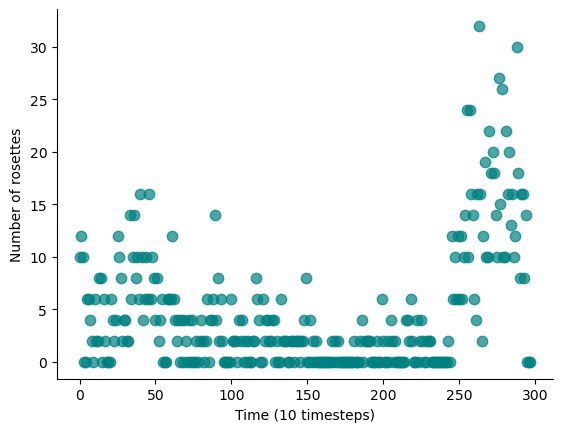
\includegraphics[width=0.5\linewidth]{chapters/Results/figures/rosettes_time.png}
    \caption{Caption}
    \label{fig:enter-label}
\end{figure}

:(

\subsection{Daniel-data?}
\newpage
\section{In Silico Mutant "predictions" - compared to phenotypes and reference model}
\subsection{No PMG}

Knocking out \dots

\begin{figure}[H]
    \centering
    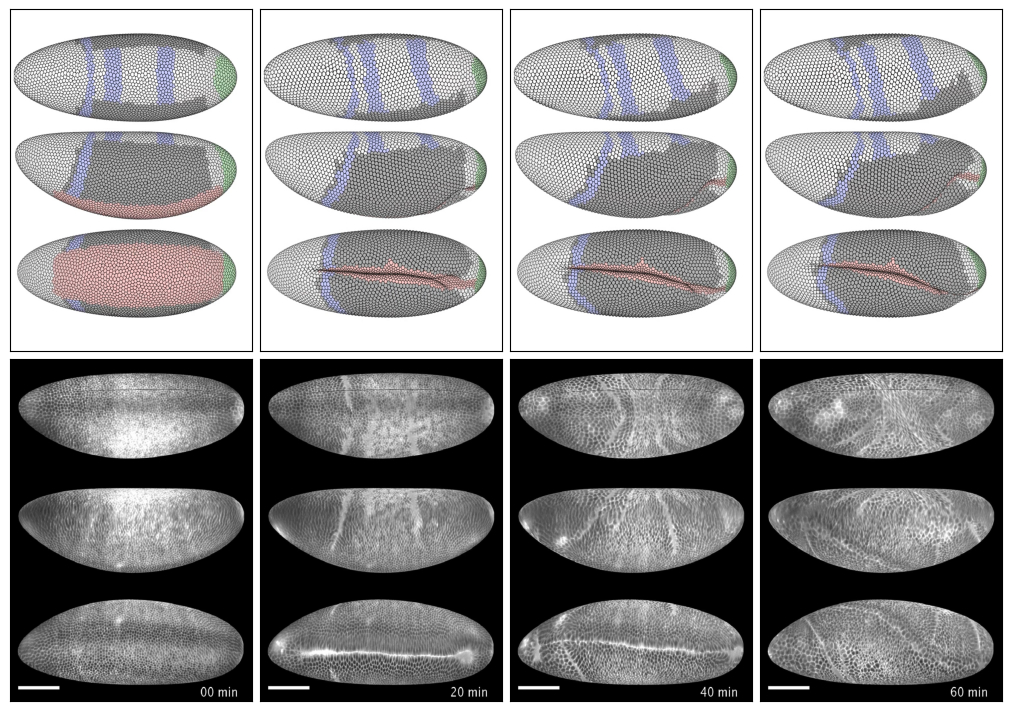
\includegraphics[width=1\linewidth]{chapters/Results/figures/corkscrew_comparison.png}
    \caption{Comparing the \textit{Corkscrew} phenotype with my simulation. Video taken from \cite{smits2023maintaining}}
    \label{fig:corkscrew-comparison}
\end{figure}
% Twist and shout
\subsection{No Ventral Furrow}
% \url{https://genesdev.cshlp.org/content/5/9/1568.full.pdf}
% We are seeing the right thing
\subsection{No Cephalic Furrow?}
% maybe not important
\subsection{No active intercolation / Germ band}
% \url{https://softmath.seas.harvard.edu/wp-content/uploads/2019/10/2009-07.pdf}
% clear that model is missing cell shape change!
\section{Additive/subtractive working together matrix}
% \subsubsection{}